\subsection{Parte I -- Análise estrutural}
\label{sec:parte1}

\subsubsection{Medidas básicas e componentes conexas}

As medidas desta subseção foram calculadas de forma exata sobre o grafo simples completo, com $n$ vértices e $m$ arestas. O grau médio é a média dos graus de todos os vértices, e a densidade é $2m/(n(n-1))$, a fração dos pares de vértices que são ligados por uma aresta. A Tabela~\ref{tab:basicas} reúne os valores.

\begin{table}[htbp]
  \centering
  \caption{Medidas básicas do grafo simples completo, calculadas de forma exata com o networkx.}
  \label{tab:basicas}
  \begin{tabular}{lr}
\toprule
 & Valor \\
\midrule
Vértices ($n$) & 105.938 \\
Arestas ($m$) & 2.316.948 \\
Grau mínimo & 1 \\
Grau máximo & 5.425 \\
Grau médio & 43,741585 \\
Densidade & 0,000413 \\
Componentes conexas & 83 \\
\bottomrule
\end{tabular}

\end{table}

Os números de vértices e de arestas coincidem com os declarados pelo SNAP~\cite{snapnets}, como esperado, já que o tratamento não removeu nenhuma aresta (Seção~\ref{sec:tratamento}). O grau médio coincide com $2m/n$, o que confere a soma dos graus com o dobro do número de arestas. O grau mínimo é 1, pois o arquivo só lista vértices que são extremo de alguma aresta. O grau máximo é muito maior que o grau médio, ou seja, há vértices com muito mais vizinhos que o típico. A densidade é inferior a um milésimo: apesar de cada imagem ter, em média, dezenas de vizinhas, o grafo é esparso, porque o número de pares possíveis cresce com $n^2$ e o de arestas não acompanha esse crescimento.

O grafo tem várias componentes conexas (Tabela~\ref{tab:basicas}). Como a maioria delas é muito pequena, a Tabela~\ref{tab:componentes} não lista cada componente: a maior aparece sozinha na primeira linha, e as demais são agrupadas por tamanho, com o número de componentes de cada tamanho. O número de componentes obtido pelo networkx foi conferido com o do igraph, e a soma dos tamanhos de todas as componentes é igual a $n$.

\begin{table}[htbp]
  \centering
  \caption{Componentes conexas do grafo simples completo agrupadas por tamanho (número de vértices): para cada tamanho, o número de componentes que o têm.}
  \label{tab:componentes}
  \begin{tabular}{rr}
\toprule
Tamanho & Componentes \\
\midrule
105.722 & 1 \\
11 & 1 \\
10 & 1 \\
8 & 1 \\
6 & 1 \\
5 & 2 \\
4 & 3 \\
3 & 13 \\
2 & 60 \\
\bottomrule
\end{tabular}

\end{table}

A Tabela~\ref{tab:componentes} mostra uma componente gigante, cujo tamanho coincide com os 105.722 vértices declarados pelo SNAP~\cite{snapnets}, e uma coleção de componentes minúsculas, a maior delas com 11 vértices e a maioria formada por pares de imagens ligadas só entre si. Essas componentes são grupos de imagens que não compartilham metadados com o restante da coleção. Como reúnem uma parcela desprezível dos vértices, a política de usar a maior componente nas medidas de distância (Seção~\ref{sec:tratamento}) praticamente não descarta informação.

\subsubsection{Distribuição de graus}

A distribuição de graus foi calculada de forma exata sobre o grafo simples completo: para cada grau $k$, contou-se o número de vértices com esse grau, e $P(k)$ é essa contagem dividida por $n$. A soma das contagens é igual a $n$, e a soma de $k$ vezes a contagem de cada grau é igual a $2m$, como deve ser.

\begin{figure}[htbp]
  \centering
  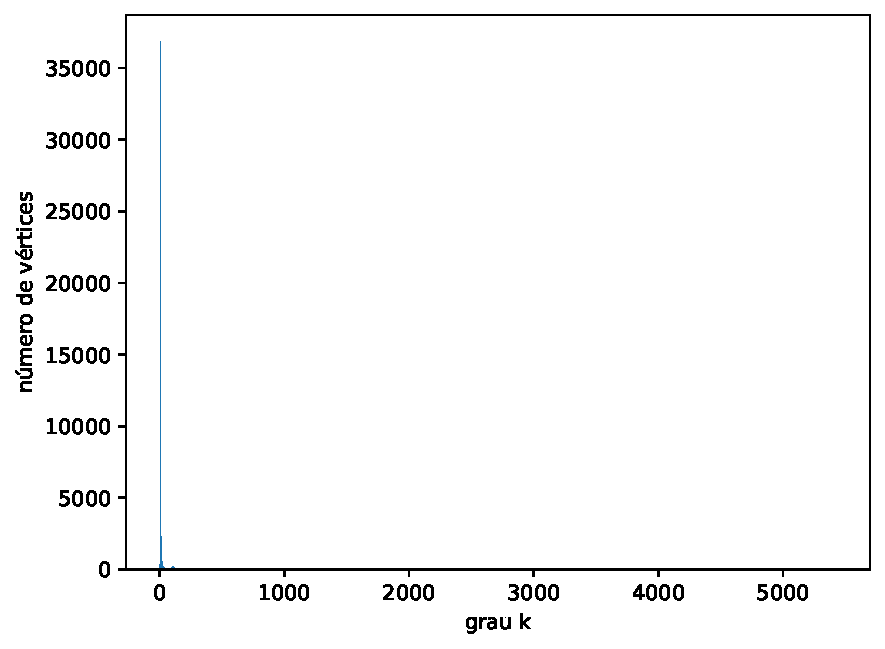
\includegraphics[width=\columnwidth]{../results/figures/graus_hist.pdf}
  \caption{Histograma dos graus do grafo simples completo em escala linear: para cada grau $k$, o número de vértices que o têm.}
  \label{fig:graus_hist}
\end{figure}

Na escala linear (Figura~\ref{fig:graus_hist}), quase toda a massa da distribuição se concentra numa barra estreita junto da origem, enquanto o eixo horizontal se estende até o grau máximo da Tabela~\ref{tab:basicas}. A distribuição é, portanto, fortemente assimétrica à direita: a maioria das imagens tem poucas vizinhas, e uns poucos vértices de grau muito alto, invisíveis nessa escala, puxam o grau médio para bem acima do grau típico.

\begin{figure}[htbp]
  \centering
  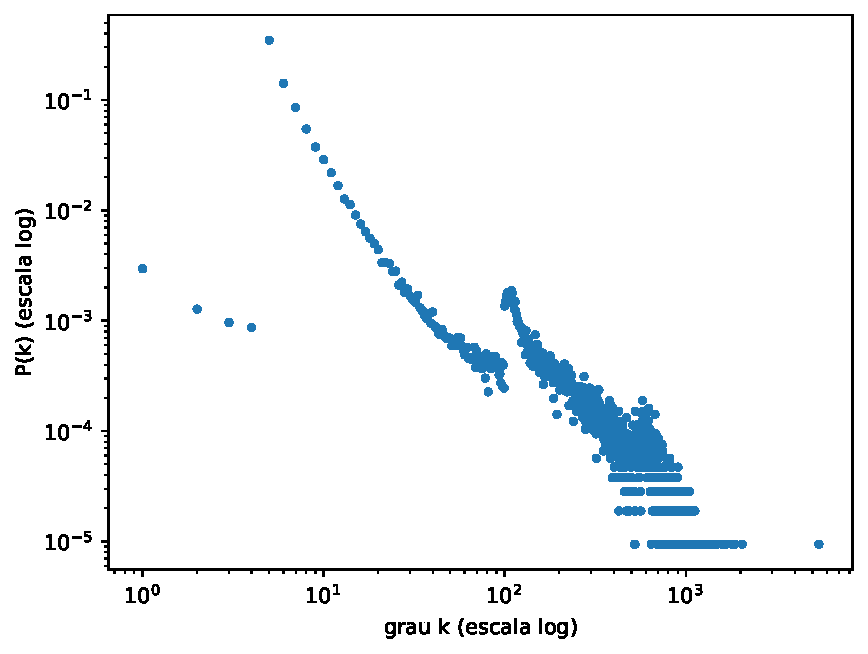
\includegraphics[width=\columnwidth]{../results/figures/graus_loglog.pdf}
  \caption{Distribuição de graus $P(k)$ do grafo simples completo em escala log-log: cada ponto é a fração dos vértices com grau $k$.}
  \label{fig:graus_loglog}
\end{figure}

A escala log-log (Figura~\ref{fig:graus_loglog}) revela o que a escala linear esconde. Os graus de 1 a 4 são raros, e o valor mais frequente é $k = 5$. A partir dele, $P(k)$ decresce de forma contínua ao longo de mais de duas ordens de grandeza de $k$, com uma elevação local perto de $k = 100$. A cauda é longa: há vértices com centenas e milhares de vizinhos, os hubs do grafo, e o de maior grau fica isolado no extremo direito, bem distante dos demais. Na cauda, muitos graus aparecem uma única vez, o que forma a faixa horizontal de pontos na base da figura. Se essa cauda segue ou não uma lei de potência é examinado na Seção~\ref{sec:parte3}.
